\documentclass[a4paper]{article}

\input{style/ch_xelatex.tex}
\input{style/scala.tex}

\usepackage[fontset=none]{ctex}
\usepackage{graphicx}
\usepackage{color,framed}
\usepackage{listings}
\usepackage{caption}
\usepackage{amssymb}
\usepackage{enumerate}
\usepackage{xcolor}
\usepackage{bm}
\usepackage{lastpage}
\usepackage{fancyhdr}
\usepackage{tabularx}
\usepackage{geometry}
\usepackage{graphics}
\usepackage{subfigure}
\usepackage{float}
\usepackage{pdfpages}
\usepackage{pgfplots}
\usepackage{multirow}
\usepackage{footnote}
\usepackage{booktabs}
\usepackage{hyperref}

\setmainfont{Times New Roman}
\setsansfont{Arial}
\setmonofont{Menlo}
\setCJKmainfont{STSong}
\setCJKsansfont{Heiti SC}
\setCJKmonofont{STSong}
\allsectionsfont{\sffamily}

\pgfplotsset{width=10cm,compat=1.9}

\lstset{
breaklines=true,
basicstyle=\small\ttfamily,
keywordstyle=\color{blue!70}\bfseries,
commentstyle=\color{red!50!green!50!blue!50},
stringstyle=\ttfamily,
extendedchars=false,
linewidth=\textwidth,
numbers=left,
numberstyle=\tiny \color{blue!50},
frame=trbl,
rulesepcolor=\color{red!20!green!20!blue!20}
}

\geometry{a4paper,left=2.3cm,right=2.3cm,top=2.7cm,bottom=2.7cm}
\pagestyle{fancy}
\lhead{\leftmark}
\rhead{PA4 实验报告}
\lfoot{}
\cfoot{\thepage}
\rfoot{}
\renewcommand{\headrulewidth}{0.1pt}
\renewcommand{\footrulewidth}{0pt}
\setlength{\textfloatsep}{8mm}
\graphicspath{{images/}{fig/}}

\begin{document}
\renewcommand{\contentsname}{目\ 录}
\renewcommand{\appendixname}{附录}
\renewcommand{\appendixpagename}{附录}
\renewcommand{\refname}{参考文献}
\renewcommand{\figurename}{图}
\renewcommand{\tablename}{表}
\renewcommand{\today}{\number\year 年 \number\month 月 \number\day 日}

\begin{titlepage}
  \begin{center}
    
\includegraphics[width=0.8\textwidth]{NKU.png}\\[1cm]
    \vspace{18mm}
    \textbf{\huge\textbf{计算机学院}}\\[0.5cm]
    \textbf{\huge{计算机系统基础（PA）实验报告}}\\[2.1cm]
    \textbf{\Huge\textbf{PA4：分页与分时多任务}}

    \vspace{\fill}
    \centering
    \textsc{\LARGE 姓名\ :\ 林晖鹏}\\[0.5cm]
    \textsc{\LARGE 学号\ :\ 2312966}\\[0.5cm]
    \textsc{\LARGE 专业\ :\ 计算机科学与技术}\\[0.5cm]

    \vfill
    {\Large \today}
  \end{center}
\end{titlepage}

\renewcommand{\thefigure}{\thesection{}.\arabic{figure}}
\renewcommand{\contentsname}{目录}
\cfoot{\thepage\ of \pageref{LastPage}}

\clearpage
\tableofcontents
\newpage

\section{概述}
PA4 继续在 PA3 的基础上往前推进。前一阶段主要解决的是系统调用、文件系统和设备接口，到了这一阶段，系统需要从能跑一个用户程序，进一步变成由操作系统管理多个进程轮流运行。围绕这个目标，实验的主线可以归结为两部分：一部分是分页机制，用来为不同进程准备彼此独立的虚拟地址空间；另一部分是硬件中断驱动的上下文切换，用来周期性夺回 CPU 并完成进程切换。

从工程实现上看，PA4 涉及的层次比 PA3 更分散：NEMU 需要支持 \texttt{CR0/CR3}、页表翻译和时钟中断；AM 需要提供 \texttt{PTE}、\texttt{\_map()}、\texttt{\_protect()}、\texttt{\_umake()} 和 trap 返回路径；Nanos-lite 需要实现物理页分配、按页装载用户程序、堆区扩展、进程管理和调度；最终还要在用户层看到 \texttt{pal}、\texttt{hello}、\texttt{videotest} 等程序分时运行。因此，PA4 更像是在做一个真正的、尽管仍然很简化的多任务操作系统。

\section{实验目的}
本次实验的目标可以概括成一条完整主线：先在 NEMU 中补齐分页相关硬件语义，让虚拟地址访问能够真正落到页表翻译上；再在 AM 与 Nanos-lite 中建立内核页表和用户页表，把用户程序的装载方式从固定物理地址拷贝改成按页分配物理页并建立映射；接着补齐 \texttt{mm\_brk()}、\texttt{\_umake()}、\texttt{schedule()} 和 \texttt{trap.S} 返回路径这几部分，使系统具备基本的进程切换能力；最后加入时钟中断，完成真正的抢占式分时多任务，并让 \texttt{pal}、\texttt{hello}、\texttt{videotest} 能够按照指导书要求运行和切换。

\section{实验内容}
结合指导书与本次真实实现过程，PA4 的内容大致沿着四个阶段展开。第一阶段是 NEMU 侧的分页硬件机制，包括控制寄存器、页表遍历和分页访存；第二阶段是在 AM 与 Nanos-lite 中建立地址空间，完成 \texttt{\_map()}、按页 \texttt{loader()} 和 \texttt{mm\_brk()}；第三阶段是把 \texttt{\_umake()}、\texttt{schedule()}、\texttt{trap.S} 和时钟中断接起来，得到真正的分时多任务；最后一阶段则是补齐 \texttt{videotest} 装载、\texttt{F12} 切换和优先级调度等展示功能。

\section{在 NEMU 中实现分页硬件机制}

\subsection{加入 \texttt{CR0/CR3} 与分页相关状态}
分页支持是从 NEMU 的 CPU 状态开始接进去的。原来的 \texttt{CPU\_state} 只有通用寄存器、\texttt{EIP} 和 \texttt{EFLAGS}，还没有页表相关状态。这里先在 \texttt{nemu/include/cpu/reg.h} 中补上 \texttt{CR0}、\texttt{CR3} 和 \texttt{INTR}：

\begin{lstlisting}[language=C]
typedef struct {
  ...
  union {
    uint32_t eflags;
    struct {
      ...
      uint32_t IF : 1;
      ...
    };
  };

  CR0 cr0;
  CR3 cr3;
  bool INTR;
} CPU_state;
\end{lstlisting}

这里的写法没有直接把 \texttt{CR0} 和 \texttt{CR3} 当成普通的 \texttt{uint32\_t}，而是继续在 \texttt{nemu/include/memory/mmu.h} 中把它们定义成带位域的联合体：

\begin{lstlisting}[language=C]
typedef union CR0 {
  struct {
    uint32_t protect_enable : 1;
    uint32_t dont_care      : 30;
    uint32_t paging         : 1;
  };
  uint32_t val;
} CR0;

typedef union CR3 {
  struct {
    uint32_t pad0                : 3;
    uint32_t page_write_through  : 1;
    uint32_t page_cache_disable  : 1;
    uint32_t pad1                : 7;
    uint32_t page_directory_base : 20;
  };
  uint32_t val;
} CR3;
\end{lstlisting}

\texttt{CR0} 这里只关心两个位：\texttt{protect\_enable} 表示处理器是否处在保护模式，\texttt{paging} 表示分页是否已经开启。后面实现 \texttt{page\_translate()} 时，代码正是通过检查这两个位来决定当前访问是否需要做页级地址转换。 \texttt{CR3} 里最有用的字段是 \texttt{page\_directory\_base}，它保存页目录物理页框号，真正用的时候再左移 12 位还原成页目录的物理基址。

有了寄存器状态之后，还需要让指令真的能够访问这些控制寄存器。这里在 \texttt{nemu/src/cpu/exec/system.c} 中补上了 \texttt{mov\_r2cr} 和 \texttt{mov\_cr2r}：

\begin{lstlisting}[language=C]
make_EHelper(mov_r2cr) {
  switch (id_dest->reg) {
    case 0: cpu.cr0.val = id_src->val; break;
    case 3: cpu.cr3.val = id_src->val; break;
    default: Assert(0, "cr%d is not implemented yet", id_dest->reg);
  }
}

make_EHelper(mov_cr2r) {
  switch (id_src->reg) {
    case 0: operand_write(id_dest, &cpu.cr0.val); break;
    case 3: operand_write(id_dest, &cpu.cr3.val); break;
    default: Assert(0, "cr%d is not implemented yet", id_src->reg);
  }
}
\end{lstlisting}

这两条指令接通以后，AM 和 Nanos-lite 才能通过正常的 x86 指令去读写控制寄存器。写 \texttt{CR3} 的效果是切换当前使用的页目录，写 \texttt{CR0} 的效果是更新分页开关。代码里只处理了 \texttt{CR0} 和 \texttt{CR3}，这是因为 PA4 现阶段真正会用到的也只有这两个控制寄存器，其它寄存器先保持未实现即可。

为了让这些状态从启动时就处在一个可控的初值上，这里还在 \texttt{nemu/src/monitor/monitor.c} 的 \texttt{restart()} 里补了初始化：

\begin{lstlisting}[language=C]
static inline void restart() {
  cpu.eip = ENTRY_START;
  cpu.cs = 0x8;
  cpu.eflags = 0x00000002;

  cpu.cr0.val = 0x00000001;
  cpu.cr3.val = 0;
  cpu.INTR = false;
}
\end{lstlisting}

\texttt{cpu.cr0.val = 0x00000001} 表示处理器先从保护模式、未开启分页的状态起步，这样前面的 PA3 代码仍然可以正常运行；\texttt{cpu.cr3.val = 0} 说明这时还没有正式切入某个有效页目录；\texttt{cpu.INTR = false} 则给后面的时钟中断轮询留出了明确的初始状态。等到 Nanos-lite 在 MM 初始化阶段真正建好内核页表之后，再通过 AM 提供的接口写入 \texttt{CR3} 并打开 \texttt{CR0.PG}，分页机制才会正式接管后续的虚拟地址访问。

这一小部分虽然改动不多，但作用很明确：它先把分页和中断需要的硬件状态接进 NEMU，再给后续的 \texttt{page\_translate()}、页表切换和定时器中断提供统一的状态入口。没有这些寄存器字段和指令支持，后面的页表代码即使写出来，也没有地方真正保存和切换处理器看到的分页状态。

\subsection{实现 \texttt{page\_translate()} 和分页访存}
分页机制真正起作用的关键，在于每次虚拟地址访问时都先经过页表翻译。因此这里在 \texttt{nemu/src/}
\texttt{memory/memory.c} 中实现了 \texttt{page\_translate()}。这一部分是按一个很直接的顺序补起来的：先判断 \texttt{CR0.PG} 是否已经开启，未开启时直接返回原地址；开启之后再从 \texttt{CR3} 取得页目录物理基址，随后按虚拟地址拆出页目录索引、页表索引和页内偏移，依次读取 \texttt{PDE} 和 \texttt{PTE}，检查 \texttt{present}，维护 \texttt{accessed/dirty}，最后再拼出真正的物理地址，并把 \texttt{vaddr\_read()/vaddr\_write()} 都接到这条翻译路径上。

核心代码结构如下：
\begin{lstlisting}[language=C]
paddr_t page_translate(vaddr_t addr, bool is_write) {
  PDE pde;
  PTE pte;
  paddr_t pdir = cpu.cr3.page_directory_base << 12;

  pde.val = paddr_read(pdir + (DIR(addr) << 2), 4);
  Assert(pde.present, "PDE not present");
  pde.accessed = 1;
  paddr_write(pdir + (DIR(addr) << 2), 4, pde.val);

  paddr_t pt = pde.page_frame << 12;
  pte.val = paddr_read(pt + (PAGE(addr) << 2), 4);
  Assert(pte.present, "PTE not present");
  pte.accessed = 1;
  if (is_write) pte.dirty = 1;
  paddr_write(pt + (PAGE(addr) << 2), 4, pte.val);

  return (pte.page_frame << 12) | OFF(addr);
}
\end{lstlisting}

这段代码可以按页级地址转换的真实顺序来读。第一句 \texttt{cpu.cr3.page\_directory\_base << 12} 先取到页目录所在的物理页；随后 \texttt{paddr\_read(pdir + (DIR(addr) << 2), 4)} 根据虚拟地址的高 10 位定位 PDE；\texttt{Assert(pde.present)} 的作用是尽早发现页目录缺项，而不是让错误拖到后面变成更难查的随机现象；接着将 \texttt{pde.accessed = 1} 写回，说明该页目录项已经被访问过。后半段对 \texttt{PTE} 做的是完全同样的事情，只不过粒度进一步下降到页表项；如果当前是写访问，还需要额外把 \texttt{dirty} 位置 1。最后一行把物理页框号和页内偏移拼接起来，得到真正落到物理内存上的地址。

分页机制落到代码里，关键就在每次访存前都要走一遍 \texttt{CR3 -> PDE -> PTE} 的解析链路。如果这里直接返回原地址，用户程序虽然写的是虚拟地址，实际仍然是在直接访问物理内存，后面每个进程拥有独立地址空间这件事也就无从谈起。

随后，这里让 \texttt{vaddr\_read()} 与 \texttt{vaddr\_write()} 真正走分页路径。对于不跨页访问，只需先翻译一次地址；对于跨页访问，则按字节拆开，逐字节完成地址翻译与读写。这种写法虽然不追求性能，但逻辑清晰，也更适合当前阶段先保证正确性。

\subsection{关键认识}
这一阶段最容易写错的地方不在语法，而在观念。\texttt{CR3}、\texttt{PDE}、\texttt{PTE} 里保存的是物理地址，不是虚拟地址；\texttt{present} 如果不检查，很多错误会在很后面才暴露；分页一旦开启，NEMU 中几乎所有虚拟地址访问都不能再直接绕过页表。做到这里之后，NEMU 已经具备了支撑分页的最小硬件语义，但系统还没有真正切到分页上运行，因为页表尚未建立，\texttt{HAS\_PTE} 也还没有打开。

\section{建立地址空间并让用户程序运行在分页机制上}

\subsection{打开 \texttt{HAS\_PTE} 与建立内核页表}
在 \texttt{nanos-lite/src/main.c} 中定义 \texttt{HAS\_PTE} 之后，系统初始化流程会先进入 \texttt{init\_mm()}，再进一步调用 AM 中的 \texttt{\_pte\_init()}。这一步会以内核可用空闲内存起始地址作为物理页分配起点，建立内核页目录和页表，设置 \texttt{CR3}，最后打开 \texttt{CR0.PG}。内核先在分页机制上跑起来，后面的用户进程地址空间才有基础。

这一部分在当前代码里的核心实现如下：
\begin{lstlisting}[language=C]
void init_mm() {
  pf = (void *)PGROUNDUP((uintptr_t)_heap.start);
  _pte_init(new_page, free_page);
}

void _pte_init(void* (*palloc)(), void (*pfree)(void*)) {
  ...
  set_cr3(kpdirs);
  set_cr0(get_cr0() | CR0_PG);
}
\end{lstlisting}

\texttt{init\_mm()} 的动作很少，但顺序很重要。第一句先把 \texttt{pf} 放到堆区页对齐后的起始位置，表示后面所有物理页都从这里顺序分配；第二句把物理页分配与回收函数传给 \texttt{\_pte\_init()}。而在 \texttt{\_pte\_init()} 内部，真正关键的是最后两句：\texttt{set\_cr3(kpdirs)} 把当前页目录切到内核页目录，\texttt{set\_cr0(get\_cr0() | CR0\_PG)} 则正式打开分页。也就是说，分页并不是单独由 NEMU 打开的，而是 AM 和 Nanos-lite 合起来把“页表已经准备好”和“处理器开始按页表访存”这两件事接上的。

\subsection{实现 \texttt{\_map()} 与按页建立映射}
接下来需要在 \texttt{nexus-am/am/arch/x86-nemu/src/pte.c} 中实现 \texttt{\_map()}。它负责把某个地址空间中的虚拟页映射到给定物理页。实现时，先从 \texttt{p->ptr} 找到页目录基址，再根据虚拟地址算出 PDE/PTE 下标；如果对应页表还不存在，就先分配一页新的页表并清零，随后填写 PDE 和 PTE，并把 \texttt{PTE\_P | PTE\_W | PTE\_U} 这些标志带上。

对应代码骨架如下：
\begin{lstlisting}[language=C]
void _map(_Protect *p, void *va, void *pa) {
  PDE *pgdir = (PDE *)p->ptr;
  uint32_t pdx = ((uintptr_t)va >> 22) & 0x3ff;
  uint32_t ptx = ((uintptr_t)va >> 12) & 0x3ff;

  if (!pgdir[pdx].present) {
    PTE *pt = (PTE *)palloc_f();
    memset(pt, 0, PGSIZE);
    pgdir[pdx].val = make_pde(pt);
  }

  PTE *pt = (PTE *)(pgdir[pdx].page_frame << 12);
  pt[ptx].val = make_pte(pa);
}
\end{lstlisting}

这段代码里，\texttt{p->ptr} 对应的是当前地址空间的页目录基址，\texttt{pdx} 和 \texttt{ptx} 则分别是虚拟地址中页目录索引和页表索引两段。第一段 \texttt{if (!pgdir[pdx].present)} 的含义是：如果目标虚拟页所在的页表还不存在，就先向物理页分配器要一页新页表，并用 \texttt{memset(pt, 0, PGSIZE)} 清零，避免旧内存残留被误解释成有效页表项；然后把这个新页表挂到 PDE 上。第二段再通过 \texttt{pgdir[pdx].page\_frame << 12} 找到对应页表，并把目标物理页写进 \texttt{pt[ptx]}。

\texttt{\_map()} 这里分成“必要时先补页表”和“再写页表项”两步，主要是为了把层次理清楚。页表本身也是普通内存对象，不会自己出现；只有先保证描述这一大片虚拟地址的页表页已经存在，后面才能继续往里面写具体虚拟页到物理页的映射关系。这个位置最容易暴露两类错误：新页表忘记清零，或者把 PDE/PTE 里的地址按虚拟地址去处理。

在这里，也顺便把新分配页必须先清零这个要求一并落实到物理页分配函数 \texttt{new\_page()} 中，因为后面用户程序按页加载、堆区补页、用户栈初始化都依赖新页内容是干净的这一前提。当前代码如下：
\begin{lstlisting}[language=C]
void* new_page(void) {
  assert(pf < (void *)_heap.end);
  void *p = pf;
  pf += PGSIZE;
  memset(p, 0, PGSIZE);
  return p;
}
\end{lstlisting}

\texttt{new\_page()} 看起来只是顺序分配一页内存，但最后的 \texttt{memset(p, 0, PGSIZE)} 非常关键。新页如果不清零，页表页里可能残留旧表项，用户栈和新堆页里也可能残留旧数据，最后出现的问题通常都不是立刻崩掉，而是很难解释的随机行为。

\subsection{把 \texttt{loader()} 改成按页加载}
PA3 中的 \texttt{loader()} 是把整个程序从 \texttt{ramdisk} 复制到固定物理地址，到了 PA4 这就不再成立了。用户程序运行在自己的虚拟地址空间中，内核也不能直接把内容写到用户虚拟地址上。因此这里把 \texttt{loader()} 改成按页工作：先为进程准备地址空间，再根据程序大小逐页循环，每次申请一页物理页，用 \texttt{\_map()} 建立虚拟页到物理页的映射，然后只把这一页对应的文件内容读进刚分配的物理页。

对应代码骨架大致如下：
\begin{lstlisting}[language=C]
for (offset = 0; offset < size; offset += PGSIZE) {
  void *pa = new_page();
  void *va = (void *)(DEFAULT_ENTRY + offset);
  _map(&pcb->as, va, pa);

  size_t len = MIN(PGSIZE, size - offset);
  fs_read(fd, pa, len);
}
\end{lstlisting}

这段循环的每一轮都在做一件很具体的事：先通过 \texttt{new\_page()} 申请一页干净的物理页，再根据 \texttt{DEFAULT\_ENTRY + offset} 算出这一页应该在用户虚拟地址空间中的位置，然后调用 \texttt{\_map(\&pcb->as, va, pa)} 建立映射关系。只有在映射建立完成之后，\texttt{fs\_read(fd, pa, len)} 才把当前这页对应的文件内容读进那一页物理内存。这里故意把文件内容读到 \texttt{pa} 而不是 \texttt{va}，原因就在于内核此时能直接可靠访问的是自己拿到的物理页，而不是用户虚拟地址。

PA4 的 \texttt{loader()} 和 PA3 的 raw loader 差别很大。PA3 只是把整段程序复制到固定地址；PA4 则需要替用户进程逐页建立虚拟页和物理页之间的对应关系。程序未来执行时访问到 \texttt{0x8048000} 附近的虚拟地址，能读到正确的指令和数据，依赖的就是这里提前完成的映射和装载。

这部分后来直接按当前工程中的真实实现写成了下面这段代码：
\begin{lstlisting}[language=C]
uintptr_t loader(_Protect *as, const char *filename) {
  int fd = fs_open(filename, 0, 0);
  size_t size = fs_filesz(fd);
  size_t off = 0;

  while (off < size) {
    void *pa = new_page();
    void *va = (void *)((uintptr_t)DEFAULT_ENTRY + off);
    size_t len = size - off;
    if (len > PGSIZE) len = PGSIZE;

    _map(as, va, pa);
    fs_read(fd, pa, len);
    off += len;
  }

  fs_close(fd);
  return (uintptr_t)DEFAULT_ENTRY;
}
\end{lstlisting}

这段代码的顺序可以直接对应装载过程来理解。第一句先通过 \texttt{fs\_open()} 和 \texttt{fs\_filesz()} 拿到目标用户程序和程序大小；随后进入按页循环，每次先申请一页物理页 \texttt{pa}，再把这页物理页映射到当前应该装入的虚拟页 \texttt{va}；长度 \texttt{len} 则控制每次最多读取一页，最后一页不足 \texttt{PGSIZE} 时只读取真实存在的那部分内容。后面的 \texttt{fs\_read(fd, pa, len)} 不是把数据读到用户虚拟地址，而是直接读到刚分配的物理页里。这样做完之后，用户程序将来访问那一页虚拟地址时，页表翻译就会把访问导向这里已经写好内容的物理页。

同时，按照讲义要求，用户程序入口和链接地址都统一改到了 \texttt{0x8048000} 附近，而不再使用 PA3 时期的 \texttt{0x4000000}。分页加载成功后，\texttt{dummy} 可以在自己的虚拟地址空间中输出 \texttt{GOOD TRAP}，如图 \ref{fig:pa4-paging-good-trap} 所示。

\begin{figure}[H]
  \centering
  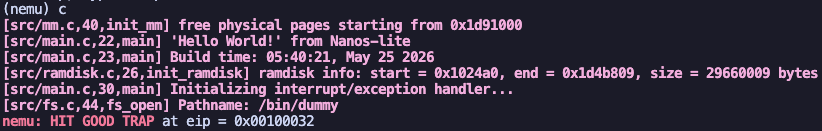
\includegraphics[width=0.82\textwidth]{pa4-paging-good-trap.png}
  \caption{分页加载后的 \texttt{dummy} 顺利输出 \texttt{GOOD TRAP}}
  \label{fig:pa4-paging-good-trap}
\end{figure}

\subsection{修复 \texttt{mm\_brk()} 与堆区映射}
分页机制引入之后，用户程序的堆区也不能再像 PA3 那样默认高地址都可以直接使用。因此这里在 \texttt{nanos-lite/src/mm.c} 中实现了按页补映射的 \texttt{mm\_brk()}。实际做法是：先在 \texttt{load\_prog()} 中初始化每个进程的 \texttt{cur\_brk/max\_brk}，之后当新的 \texttt{brk} 超过旧边界时，就从旧边界开始按页补映射，每补一页都调用 \texttt{\_map(\&current->as, ...)} 建立新的页表项。

这一部分调试时还顺手修掉了两个很要命的隐患。其一是 \texttt{mm\_brk()} 第一次调用时不能只更新 \texttt{cur\_brk/max\_brk} 而不补映射，否则首次申请出来的堆区根本不可访问；其二是 \texttt{new\_page()} 必须把新页清零，不然程序末页、用户栈和新堆页都会带着脏数据。

\texttt{mm\_brk()} 的实际代码思路也是按页增长，而不是一次性修改最大堆顶：
\begin{lstlisting}[language=C]
int mm_brk(uintptr_t new_brk) {
  uintptr_t brk = PGROUNDUP(current->max_brk);
  while (brk < new_brk) {
    _map(&current->as, (void *)brk, new_page());
    brk += PGSIZE;
  }
  current->max_brk = new_brk;
  current->cur_brk = new_brk;
  return 0;
}
\end{lstlisting}

这段代码里，第一句 \texttt{PGROUNDUP(current->max\_brk)} 的作用是把当前堆顶向上取整到页边界，因为页表映射只能按整页建立；接着 \texttt{while (brk < new\_brk)} 逐页遍历这次新扩展出来的地址范围，每一轮都调用 \texttt{\_map()} 给当前进程补上一页新的堆页；循环结束后，再把 \texttt{max\_brk} 和 \texttt{cur\_brk} 更新为新的 break。换句话说，这里的元数据更新是放在实际内存补齐之后做的，而不是反过来。

\texttt{brk} 的语义不是简单把一个边界值改大，而是从当前时刻开始，这一段虚拟地址应当真的可访问。如果只更新边界值不补映射，\texttt{malloc} 或资源加载逻辑第一次写到这段地址时就会落到未映射页面上。这也是这一阶段调试里最典型的一类现象：边界值已经更新，真实访问却仍然失败。

当前 \texttt{mm\_brk()} 的实现如下：
\begin{lstlisting}[language=C]
int mm_brk(uint32_t new_brk) {
  if (new_brk > current->max_brk) {
    uintptr_t brk = PGROUNDUP(current->max_brk);
    while (brk < new_brk) {
      _map(&current->as, (void *)brk, new_page());
      brk += PGSIZE;
    }
    current->max_brk = new_brk;
  }

  current->cur_brk = new_brk;
  return 0;
}
\end{lstlisting}

\texttt{current->max\_brk} 记录的是当前已经完成映射的堆顶边界，因此只有当 \texttt{new\_brk} 超过它时，才真的需要继续补页。循环里的 \texttt{PGROUNDUP(current->max\_brk)} 把起点抬到页边界，后面的 \texttt{\_map(..., new\_page())} 则是一页一页补上映射关系。最后再更新 \texttt{max\_brk} 和 \texttt{cur\_brk}，这样边界值和真实映射状态才能保持一致。

\subsection{为什么必须把用户程序入口改到 \texttt{0x8048000}}
最开始虽然分页主线已经大体接通，但运行现象非常诡异：调度器看起来在 \texttt{pal} 和 \texttt{hello} 之间切换，时钟中断也在工作，可实际表现却像始终只有 \texttt{hello} 在跑，图形窗口只是黑屏。

继续排查后定位到根因：如果用户程序仍然链接并装载在 \texttt{0x4000000}，而内核页表又共享低地址恒等映射，那么不同用户程序很容易在这一区域上彼此覆盖。于是这里按照讲义要求，把 \texttt{navy-apps/}\\\texttt{Makefile.compile} 中的 \texttt{-Ttext 0x4000000} 改为 \texttt{-Ttext 0x8048000}，同时把 \texttt{nanos-lite/}\texttt{src/loader.c} 中的 \texttt{DEFAULT\_ENTRY} 也同步改成 \texttt{0x8048000}。

这里真正改动到的代码很直接：
\begin{lstlisting}[language=C]
#define DEFAULT_ENTRY ((void *)0x8048000)
\end{lstlisting}

虽然表面上只是把一个常量改了，但它直接影响了用户程序在虚拟地址空间中的整体布局。入口地址改到 \texttt{0x8048000} 之后，\texttt{pal}、\texttt{hello} 和 \texttt{videotest} 才能稳定地各自落在独立的用户空间区域里，避免在低地址区发生覆盖。

修改之后，\texttt{pal} 才真正开始运行在自己的用户虚拟地址空间上，并进入初始化流程，如图 \ref{fig:pa4-pal-startup} 所示。

\begin{figure}[H]
  \centering
  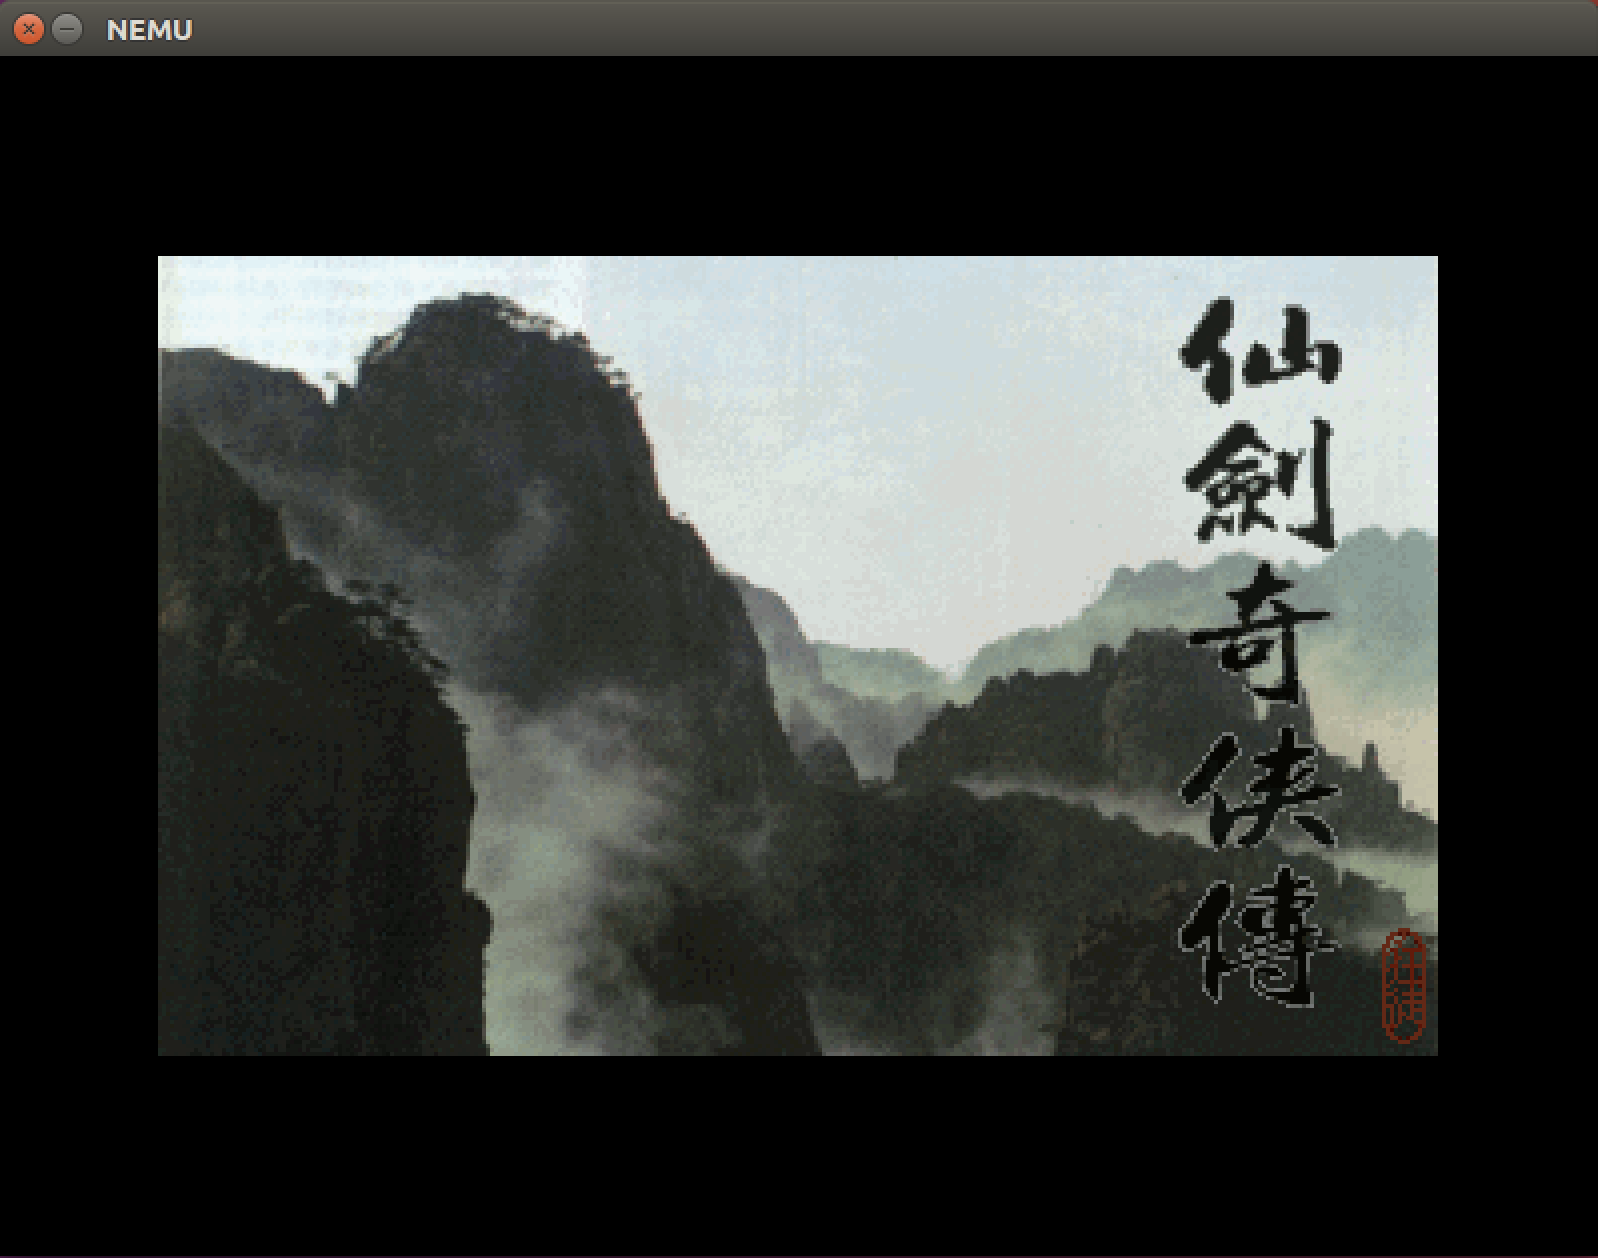
\includegraphics[width=0.82\textwidth]{pa4-pal-startup.png}
  \caption{\texttt{pal} 已经在分页机制下启动并开始初始化资源}
  \label{fig:pa4-pal-startup}
\end{figure}

\section{上下文切换、时钟中断与真正的分时多任务}

\subsection{构造新进程初始现场：\texttt{\_umake()}}
分页和地址空间打通之后，还不能直接得到多任务能力，因为新进程第一次运行时并没有真实经历过异常陷入。为了解决这个问题，AM 中的 \texttt{\_umake()} 负责在内核栈上人工构造一份可被恢复的 trap frame。这里至少要把 \texttt{eip} 设为程序入口，把 \texttt{cs} 设为 \texttt{0x8}，把 \texttt{eflags} 设成 \texttt{0x202} 以保证 \texttt{IF = 1}，同时还要准备好用户栈顶和用户态 \texttt{\_start()} 需要看到的初始栈布局。

只有当这份初始现场布置正确后，调度器未来切换到该进程时，\texttt{trap.S} 才能像处理中断返回现场那样，把它恢复出来并开始执行。

把这一段落实到代码上，一个典型的 \texttt{\_umake()} 骨架可以写成：
\begin{lstlisting}[language=C]
tf->eip = (uintptr_t)entry;
tf->cs = 0x8;
tf->eflags = 0x202;
tf->esp = (uintptr_t)ustack.end;

ustack.end[-1] = 0;
ustack.end[-2] = (uintptr_t)argv;
ustack.end[-3] = argc;
ustack.end[-4] = 0;
\end{lstlisting}

前四行是在构造未来会被 \texttt{iret} 恢复出来的关键寄存器现场。把 \texttt{eip} 设成程序入口，意味着这个进程第一次真正运行时会从用户程序入口开始执行；\texttt{cs = 0x8} 则与当前 AM/NEMU 的代码段约定保持一致；\texttt{eflags = 0x202} 最关键的地方在于把 \texttt{IF} 位置 1，否则用户态运行期间根本无法响应时钟中断；\texttt{esp} 被放到用户栈顶，保证恢复后用户程序看到的是一份合法栈。

后四行则是在用户栈上伪造 \texttt{\_start()} 期望的初始参数布局。虽然这些值看上去只是几个普通槽位，但它们的作用非常关键：用户程序并不是直接从某个裸入口开始执行，而是仍然期望看到一份像正常 C 运行时那样的参数环境。因此，\texttt{\_umake()} 并不只是填几个寄存器，而是在人工构造一份可直接返回到用户态的初始现场。也正因为这份现场足够完整，调度器第一次切到该进程时，\texttt{trap.S} 才能像平时处理中断返回那样，直接把它恢复出来运行。

而用户栈本身是在 \texttt{load\_prog()} 中提前准备好的，当前实现是：
\begin{lstlisting}[language=C]
uintptr_t *sp = (uintptr_t *)((uint8_t *)ustack_top_pa + PGSIZE);
*--sp = 0;
*--sp = 0;
*--sp = 0;
*--sp = 0;
\end{lstlisting}

这四个槽位从上到下分别对应 \texttt{envp}、\texttt{argv}、\texttt{argc} 和一个假的返回地址。这样做之后，用户程序第一次恢复出来时看到的栈布局就和正常 C 运行时入口保持一致，后面即使没有传参数，也不会因为初始栈完全是垃圾数据而在一开始就跑偏。

\subsection{实现 \texttt{schedule()} 与 \texttt{trap.S} 中的切栈恢复}
Nanos-lite 中的 \texttt{schedule(prev)} 做的事情并不复杂：先保存当前进程的 \texttt{tf}，再选择下一个要运行的进程，随后切换到该进程的地址空间，最后返回目标进程的 \texttt{tf}。

真正把上下文切换落实到寄存器和栈上的位置在 \texttt{trap.S}。这里的关键点是：\texttt{irq\_handle()} 返回的不是当前进程的 trap frame，而是下一个进程的 trap frame 指针。因此在 \texttt{trap.S} 中，\texttt{call irq\_handle} 返回后必须先执行：
\begin{lstlisting}[language={[x86masm]Assembler}]
movl %eax, %esp
\end{lstlisting}
然后再 \texttt{popal}、恢复段寄存器并 \texttt{iret}。这一步的本质是先切到另一个进程的栈，再按那个栈里的现场恢复寄存器。如果没有这一步，调度器就算在 C 层选中了别的 PCB，CPU 最终也还是会沿着旧进程的栈继续返回。

如果把这一段再落到代码层来看，\texttt{schedule()} 的核心骨架大致可以写成：
\begin{lstlisting}[language=C]
_RegSet* schedule(_RegSet *prev) {
  current->tf = prev;
  current = pick_next();
  _switch(&current->as);
  return current->tf;
}
\end{lstlisting}

第一句 \texttt{current->tf = prev} 的含义，是把这次被打断时保存下来的现场挂回当前 PCB 中，确保这个进程以后还能从这里继续运行；\texttt{pick\_next()} 代表调度器选择下一个进程，这里可以是简单轮转，也可以是后面加入优先级之后的版本；\texttt{\_switch(\&current->as)} 负责切换页表，让后续恢复出来的进程回到它自己的虚拟地址空间；最后返回的不是某个普通值，而是下一个进程 trap frame 的地址。

这也正是为什么 \texttt{trap.S} 必须配合完成最后一步。对应的返回路径骨架可以概括成：
\begin{lstlisting}[language={[x86masm]Assembler}]
call irq_handle
movl %eax, %esp
popal
addl $8, %esp
iret
\end{lstlisting}

\texttt{call irq\_handle} 返回到 \texttt{\%eax} 的，正是 \texttt{schedule()} 最终选中的 trap frame 指针；\texttt{movl \%eax, \%esp} 会把栈顶直接切到新进程保存现场的位置；后面的 \texttt{popal}、跳过异常号与错误码、再执行 \texttt{iret}，都因此变成了从新进程的栈中恢复寄存器并返回。上下文切换不能只靠修改 \texttt{current} 完成，CPU 最终还要真的从另一份保存现场继续执行。C 代码负责决定切给谁，汇编返回路径负责把这个决定落实到寄存器和栈上。

当前工程里的 \texttt{schedule()} 已经不是抽象骨架，而是直接带着三进程调度和优先级逻辑：
\begin{lstlisting}[language=C]
if (nr_proc >= 3) {
  PCB *game = &pcb[current_game == 0 ? 0 : 2];
  PCB *hello = &pcb[1];
  if (current == hello) {
    current = game;
    game_slice_count = 1;
  } else if (game_slice_count < GAME_SLICE_BUDGET) {
    current = game;
    game_slice_count++;
  } else {
    current = &pcb[1];
    game_slice_count = 0;
  }
}
\end{lstlisting}

这段代码说明调度器在当前版本里并不是简单轮转。它会先根据 \texttt{current\_game} 确定当前图形进程到底是 \texttt{pal} 还是 \texttt{videotest}，然后让图形进程连续跑若干个时间片，再偶尔切一次 \texttt{hello}。因此前面看到的“游戏更流畅、hello 仍然持续输出”并不是现象描述，而是这段调度逻辑直接带来的结果。

\subsection{加入时钟中断，建立抢占式调度}
如果只靠系统调用返回点进行切换，那么一旦某个用户程序长时间不主动陷入内核，系统就无法再夺回控制权。因此 PA4 还必须加入时钟中断，使调度真正由硬件时钟驱动。

本次实现中，时钟中断链路是从硬件侧一路往上接起来的：先让 NEMU 的 \texttt{timer\_intr()} 定期触发，再由 \texttt{dev\_raise\_intr()} 把 \texttt{cpu.INTR} 置高；随后 \texttt{exec\_wrapper()} 在每条指令后检查 \texttt{INTR \&\& IF}，条件满足时触发 32 号中断；\texttt{raise\_intr()} 负责保存现场并清 \texttt{IF}；AM 再在 \texttt{trap.S/asye.c} 中把它包装成 \texttt{\_EVENT\_IRQ\_TIME}；最后 Nanos-lite 在 \texttt{do\_event()} 中收到该事件后直接调用 \texttt{schedule()}。

NEMU 侧最关键的代码实际上就是这几行：
\begin{lstlisting}[language=C]
if (cpu.INTR && cpu.eflags.IF) {
  cpu.INTR = false;
  raise_intr(0x20, cpu.eip);
}
\end{lstlisting}

这几行代码虽然短，但它们是抢占式调度真正成立的前提。\texttt{cpu.INTR} 表示外部设备已经把中断请求送到了 CPU，\texttt{cpu.eflags.IF} 则表示当前处理器是否允许响应可屏蔽中断；只有两者同时为真，NEMU 才会把这次请求真正转化成一次异常入口调用。进入中断前先把 \texttt{cpu.INTR = false} 清掉，是为了避免同一次中断请求被重复处理；随后调用 \texttt{raise\_intr(0x20, cpu.eip)}，则表示从当前这条指令之后的位置开始被打断，并转入 32 号时钟中断入口。

把这段检查放在 \texttt{exec\_wrapper()} 的末尾之后，每执行完一条指令都会经过这里一次。不管当前跑的是 \texttt{pal}、\texttt{hello} 还是 \texttt{videotest}，只要时钟到了，CPU 就一定有机会被操作系统重新夺回，调度也不再依赖用户程序自己是否愿意陷入内核。

当前 NEMU 中的轮询代码如下：
\begin{lstlisting}[language=C]
if (cpu.INTR && cpu.IF) {
  cpu.INTR = false;
  raise_intr(TIMER_IRQ, cpu.eip);
  update_eip();
}
\end{lstlisting}

这里的条件判断同时检查了 \texttt{INTR} 和 \texttt{IF}。前者表示外部设备已经把中断请求送到 CPU，后者表示当前处理器仍处在开中断状态。两者都满足时，先把 \texttt{cpu.INTR} 清掉，避免同一轮中断被重复处理，再通过 \texttt{raise\_intr(TIMER\_IRQ, cpu.eip)} 把控制流送入中断入口。最后调用一次 \texttt{update\_eip()}，让前面刚刚设置好的跳转真正生效。时钟中断能够稳定插入到任何用户程序执行过程中，依赖的就是这一小段公共路径代码。

中断到了 Nanos-lite 这一层以后，真正接住它的是 \texttt{do\_event()}：
\begin{lstlisting}[language=C]
static _RegSet* do_event(_Event e, _RegSet* r) {
  switch (e.event) {
    case _EVENT_TRAP: return schedule(r);
    case _EVENT_IRQ_TIME: return schedule(r);
    case _EVENT_SYSCALL: return do_syscall(r);
    default: panic("Unhandled event ID = %d", e.event);
  }
}
\end{lstlisting}

这段代码把 PA4 的三类关键入口摆得很清楚。\texttt{\_EVENT\_SYSCALL} 继续走系统调用处理；\texttt{\_EVENT\_TRAP} 可以把内核自陷接入调度；而时钟中断对应的 \texttt{\_EVENT\_IRQ\_TIME} 直接调用 \texttt{schedule(r)}。从这里开始，调度就不再依赖用户程序自己调用系统调用，而是由硬件时钟定期推动。

运行日志中可以持续看到 \texttt{exec\_wrapper irq[...]}、\texttt{do\_event time[...]} 和 \texttt{schedule[...]}，说明时钟中断已经稳定驱动起了进程切换。对应截图如图 \ref{fig:pa4-timer-log} 所示。

\begin{figure}[H]
  \centering
  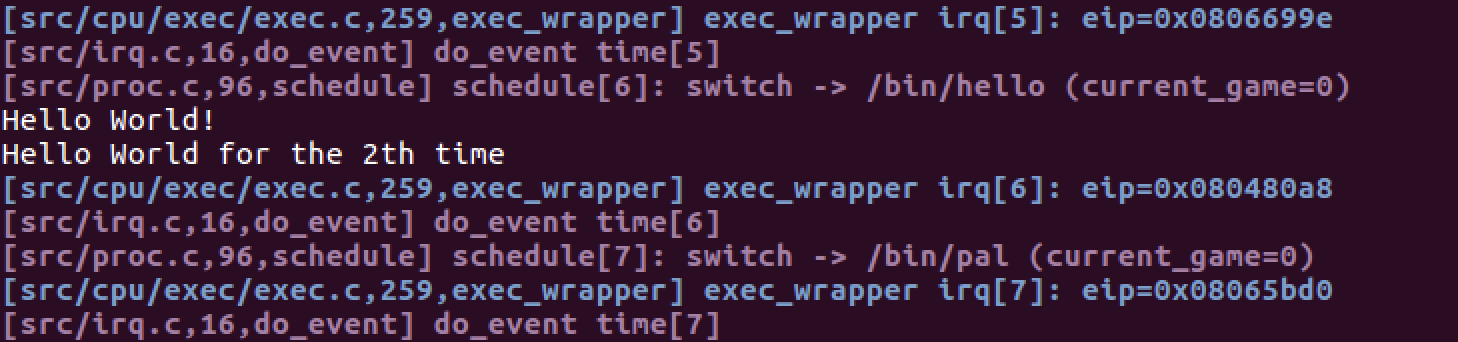
\includegraphics[width=0.84\textwidth]{pa4-timer-log.png}
  \caption{时钟中断持续触发，并通过 \texttt{\_EVENT\_IRQ\_TIME} 驱动调度}
  \label{fig:pa4-timer-log}
\end{figure}

\subsection{验证 \texttt{pal + hello} 的分时运行}
在时钟中断和上下文切换主线都接通之后，系统已经能够让 \texttt{pal} 和 \texttt{hello} 同时参与调度。此时可以看到一边有 \texttt{hello} 在终端持续输出，另一边 \texttt{pal} 也在初始化并持续运行，如图 \ref{fig:pa4-pal-hello-timeslice} 所示。

\begin{figure}[H]
  \centering
  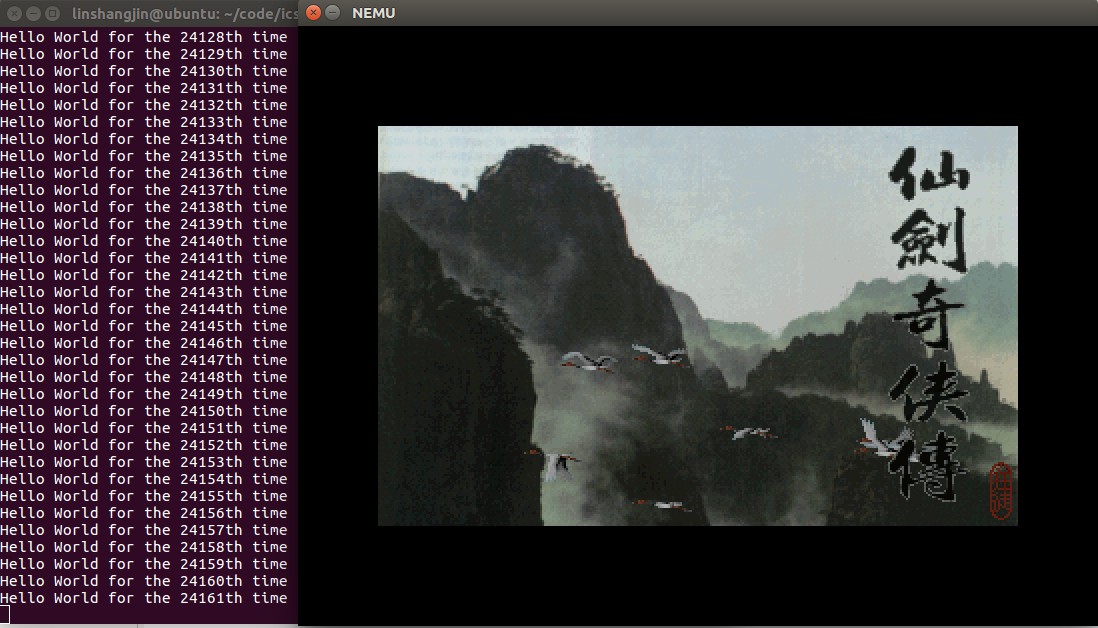
\includegraphics[width=0.76\textwidth]{pa4-pal-hello-timeslice.png}
  \caption{\texttt{pal} 与 \texttt{hello} 已经能够在时钟中断驱动下分时运行}
  \label{fig:pa4-pal-hello-timeslice}
\end{figure}

\subsection{加入优先级调度，降低 \texttt{hello} 对图形程序性能的影响}
PA4 讲义中特别提到：虽然 \texttt{hello} 和 \texttt{pal} 已经可以分时运行，但严格按 \texttt{1:1} 切换会明显拖慢游戏进程。为此，这里在 \texttt{schedule()} 中引入了轻量级优先级调度：这里定义了 \texttt{GAME\_SLICE\_BUDGET = 5}，让当前图形进程连续运行 5 个时间片，再让 \texttt{hello} 运行 1 个时间片。

对应的代码就是前面调度器里的这一段判断：
\begin{lstlisting}[language=C]
if (current == hello) {
  current = game;
  game_slice_count = 1;
} else if (game_slice_count < GAME_SLICE_BUDGET) {
  current = game;
  game_slice_count++;
} else {
  current = hello;
  game_slice_count = 0;
}
\end{lstlisting}

\texttt{game\_slice\_count} 在这里起到计数器的作用。只要当前还没达到预算上限，就继续把时间片给图形进程；达到上限之后才切一次 \texttt{hello}，然后再重新开始下一轮计数。这样既能保证 \texttt{hello} 继续输出，也能明显减轻它对图形程序性能的影响。

这样做之后，\texttt{hello} 仍然能够持续输出，证明它没有被饿死；但输出频率明显下降，\texttt{pal} 或 \texttt{videotest} 的画面流畅度比严格 \texttt{1:1} 时更好。这一部分虽然不再改变系统结构，却使得最终展示效果明显更符合实验要求。

\section{展示功能完善}

\subsection{加载 \texttt{videotest} 并实现 \texttt{F12} 切换}
指导书最后还要求实现一个展示场景：除了 \texttt{pal} 和 \texttt{hello} 之外，再额外加载 \texttt{videotest}，并允许按 \texttt{F12} 在两个图形进程之间切换。

为此，这里在 \texttt{nanos-lite/src/main.c} 中加入了：
\begin{lstlisting}[language=C]
load_prog("/bin/videotest");
\end{lstlisting}
再在 \texttt{nanos-lite/src/device.c} 中识别 \texttt{F12} 事件，并在按下时翻转 \texttt{current\_game}。调度器则根据 \texttt{current\_game} 决定当前图形时间片分配给 \texttt{pal} 还是 \texttt{videotest}，而 \texttt{hello} 始终作为后台进程保留。

\texttt{F12} 切换本身对应的代码也很短：
\begin{lstlisting}[language=C]
if (key == _KEY_F12 && down) {
  current_game = (current_game == 0 ? 1 : 0);
}
\end{lstlisting}

这里没有直接在按键处理函数里做复杂调度，而只是把 \texttt{current\_game} 翻转一下。这样做的好处是输入处理和调度逻辑仍然分开：设备层只负责记录“当前应该展示哪个图形进程”，真正何时切换、切给谁，仍然由后面的 \texttt{schedule()} 在时钟中断到来时统一决定。

修正之后，默认状态是 \texttt{pal + hello}，按下 \texttt{F12} 后可以切换为 \texttt{videotest + hello}。切换前后的界面分别如图 \ref{fig:pa4-pal-hello-before-f12} 和图 \ref{fig:pa4-videotest-after-f12} 所示。

\begin{figure}[H]
  \centering
  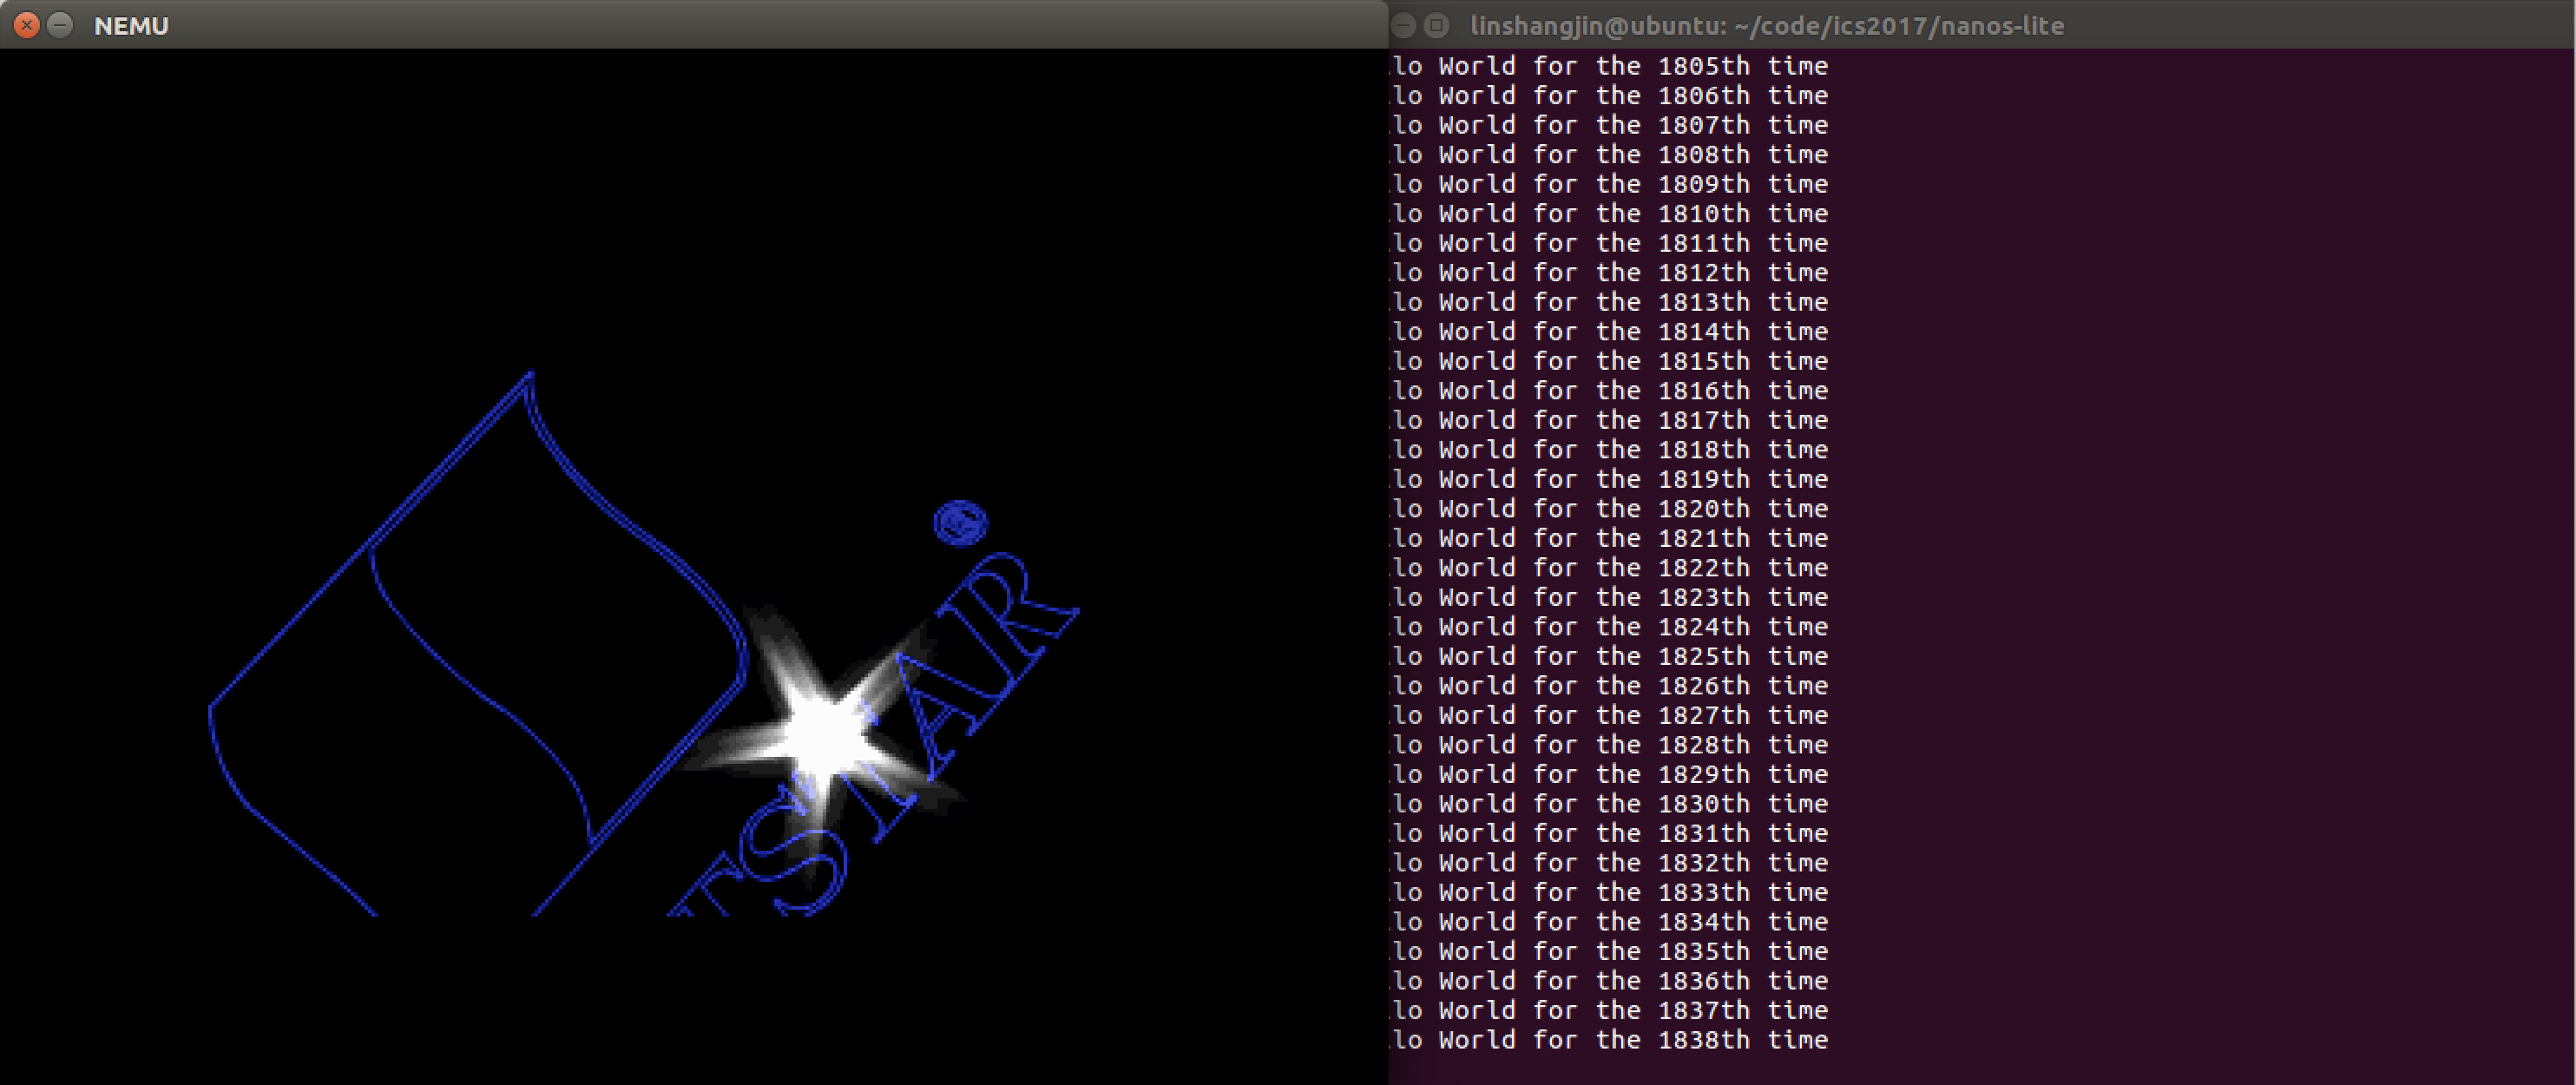
\includegraphics[width=0.74\textwidth]{pa4-pal-hello-before-f12.png}
  \caption{默认状态下的 \texttt{pal + hello}}
  \label{fig:pa4-pal-hello-before-f12}
\end{figure}

\begin{figure}[H]
  \centering
  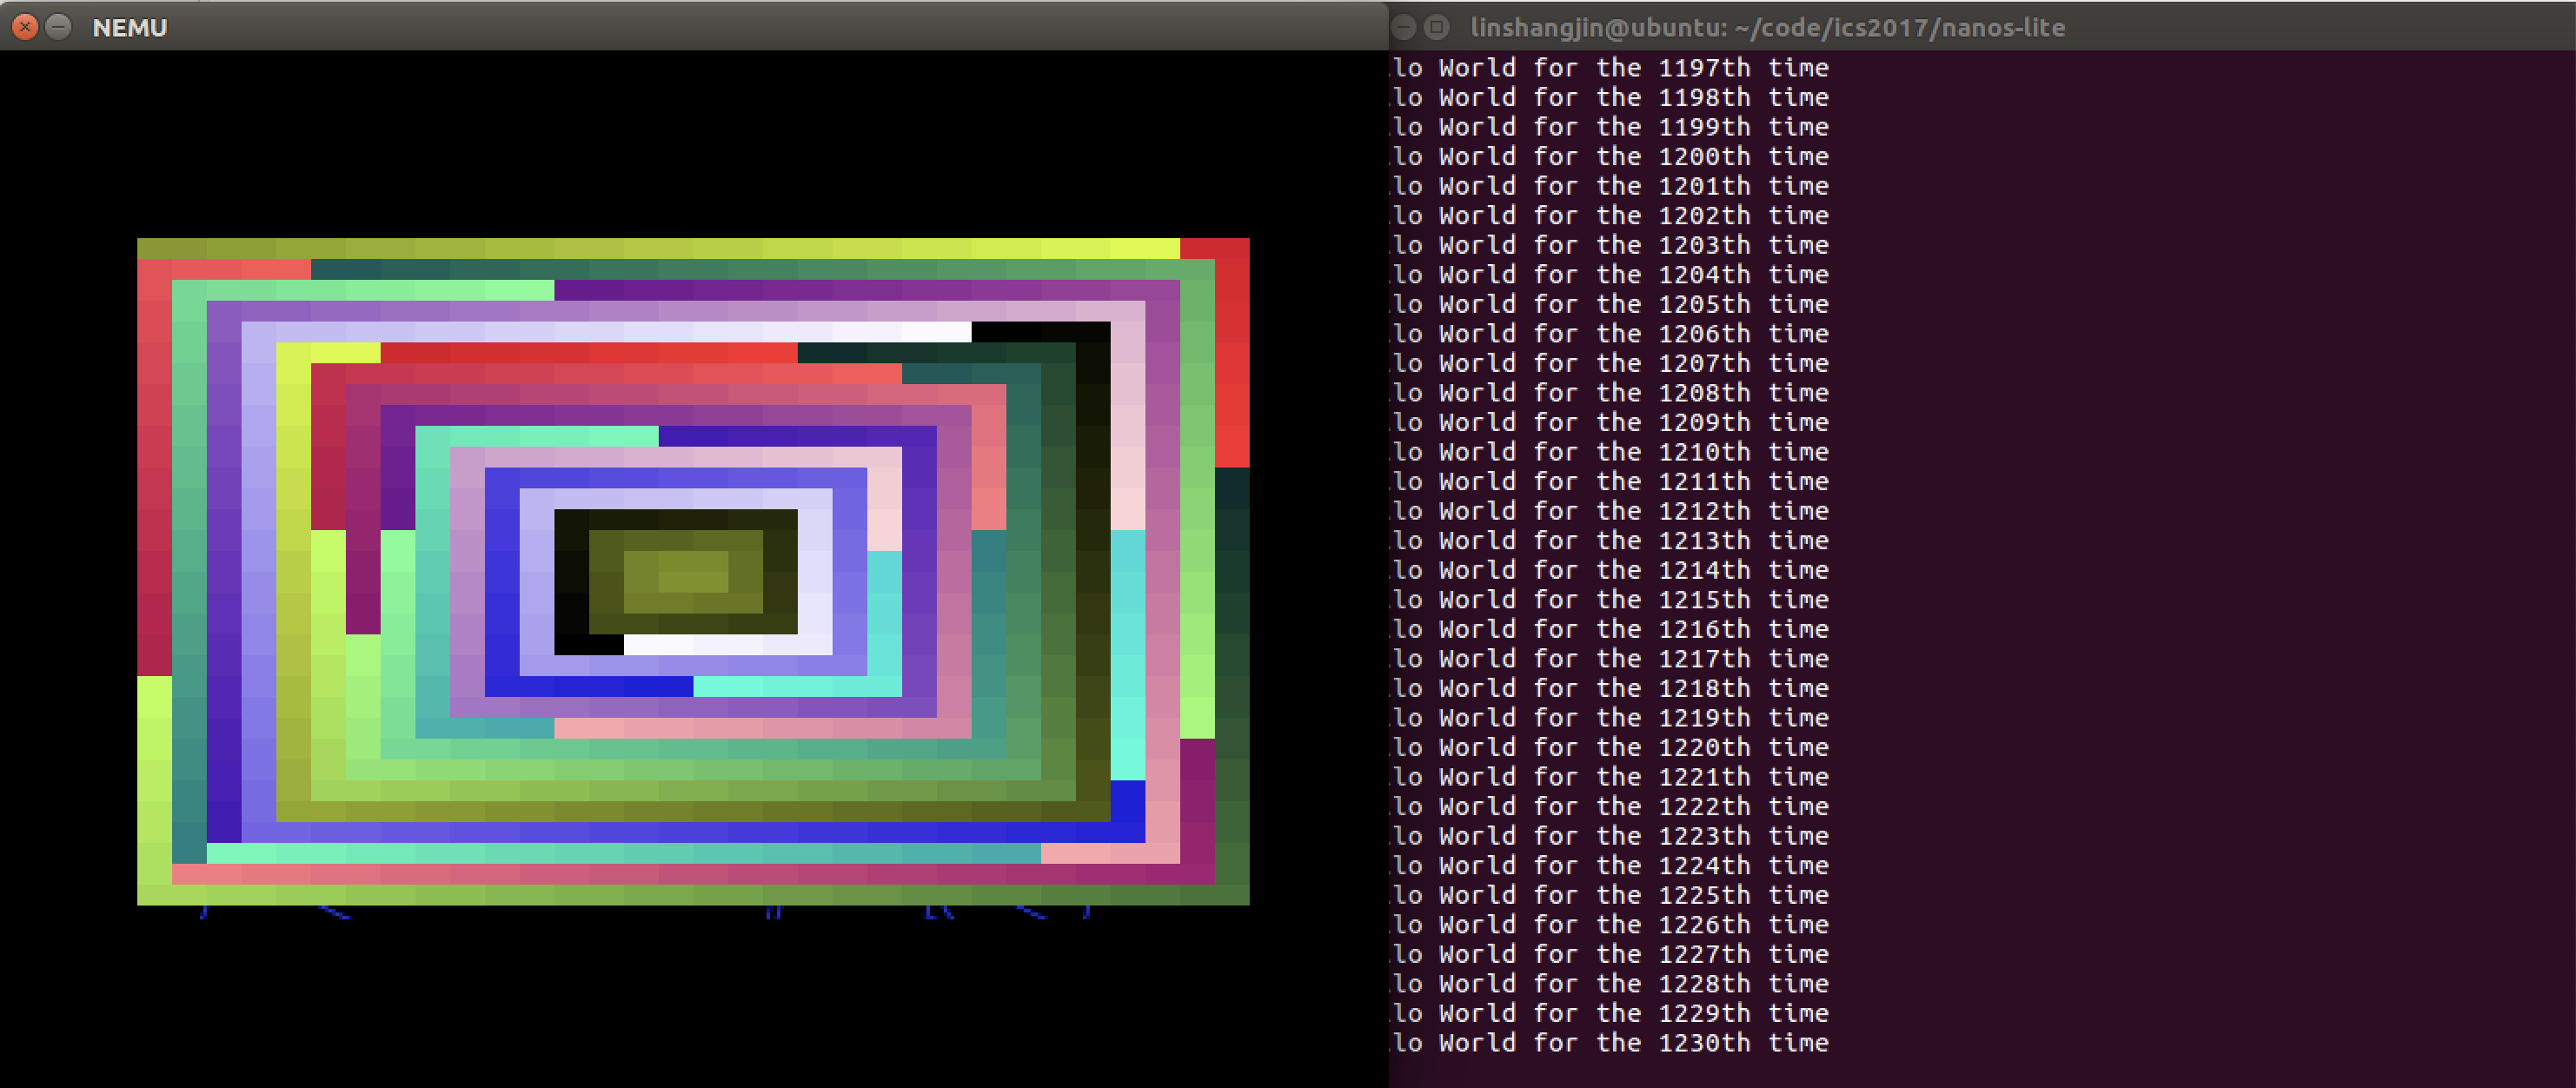
\includegraphics[width=0.74\textwidth]{pa4-videotest-after-f12.png}
  \caption{按下 \texttt{F12} 后切换到 \texttt{videotest + hello}}
  \label{fig:pa4-videotest-after-f12}
\end{figure}

\section{必答题与分析}

\subsection{分页机制和硬件中断是如何共同支撑 \texttt{pal} 与 \texttt{hello} 分时运行的}
这道题是 PA4 的核心。要完整回答它，不能只讲分页，也不能只讲中断，因为这两套机制分别解决的是不同问题：
\textbf{分页机制}解决多个进程如何拥有彼此独立的内存视图，\textbf{硬件中断}解决操作系统如何在运行过程中周期性夺回 CPU 控制权。两者少掉任何一个，\texttt{pal} 和 \texttt{hello} 都不可能稳定地分时运行。

\subsubsection{分页机制负责隔离地址空间}
如果没有分页，那么 \texttt{pal} 和 \texttt{hello} 都只能被直接装到某个固定物理地址上运行。只要同时加载两个程序，它们的数据和代码就一定会互相覆盖。因此，PA4 先用分页机制为每个进程构造独立地址空间。Nanos-lite 通过 \texttt{\_protect()} 为每个 PCB 创建一套页目录，再由 \texttt{loader()} 按页为用户程序分配物理页，\texttt{\_map()} 负责把用户虚拟地址映射到这些物理页，最后在运行该进程之前，由 \texttt{\_switch()} 把 \texttt{CR3} 切到它自己的页目录。

这样一来，\texttt{pal} 和 \texttt{hello} 虽然都认为自己运行在例如 \texttt{0x8048000} 这样的固定虚拟地址附近，但在页表转换之后，它们实际访问到的却是完全不同的物理页。也就是说，分页机制保证了多进程并存而互不覆盖。

这一步在代码层的对应关系也很直接。NEMU 的 \texttt{page\_translate()} 负责真正完成虚拟地址到物理地址的转换，AM 的 \texttt{\_map()} 负责把虚拟页与物理页的对应关系写进页表，Nanos-lite 的 \texttt{load\_prog()} 与 \texttt{mm\_brk()} 则在程序装载和堆区扩展时持续建立这些映射。

\subsubsection{硬件中断负责把 CPU 从当前进程手里抢回来}
即使地址空间隔离已经成立，如果系统仍然只有当前进程主动系统调用时才切换这一种时机，那么一旦某个程序长时间不陷入内核，另一个程序就永远得不到运行机会。因此，PA4 还必须加入时钟中断，使操作系统即使在用户程序不主动让出 CPU 的情况下，也能强行夺回控制权。

这条链路在本次实验中的实现过程也比较清楚：NEMU 的定时器先定期触发，\texttt{dev\_raise\_intr()} 把 \texttt{cpu.INTR} 拉高，\texttt{exec\_wrapper()} 每执行完一条指令都检查一次 \texttt{INTR} 和 \texttt{IF}，若允许响应中断就调用 \texttt{raise\_intr(0x20, cpu.eip)}；随后 AM 在 \texttt{trap.S} 和 \texttt{asye.c} 中把这次中断包装成 \texttt{\_EVENT\_IRQ\_TIME}，Nanos-lite 再在 \texttt{do\_event()} 中收到该事件后直接调用 \texttt{schedule()}。

硬件中断在这里提供的是一个\textbf{稳定且周期性的切入点}。内核拿到这个切入点之后，才能暂停当前进程、检查系统状态并切换到其他进程。

\subsubsection{上下文切换把两者真正连起来}
分页和时钟中断分别解决了隔离内存和夺回控制权两个问题，但要让 \texttt{pal} 与 \texttt{hello} 真的轮流运行，还必须把它们用上下文切换连起来。这里的连接方式很直接：\texttt{\_umake()} 先为新进程伪造初始现场，\texttt{schedule()} 保存当前进程的 trap frame 并选出下一个 PCB，\texttt{\_switch()} 切换到下一个进程的地址空间，最后 \texttt{trap.S} 用 \texttt{movl \%eax, \%esp} 切到新进程的 trap frame，再通过 \texttt{iret} 返回。

这意味着每次时钟中断到来时，内核都会先在当前进程的内核栈上保存一份 trap frame，再把调度器选出来的另一个进程的 trap frame 当成返回目标。于是从汇编返回之后，CPU 恢复出来的就不再是原来的寄存器现场，而是另一个进程的寄存器现场。由于同时也切换了 \texttt{CR3}，这个新现场后续访问到的内存也会自动落入它自己的虚拟地址空间中。

\subsubsection{为什么两者缺一不可}
如果只有分页、没有时钟中断，那么虽然 \texttt{pal} 和 \texttt{hello} 拥有独立地址空间，但 CPU 仍然会长期停留在某一个进程里，系统不具备真正的分时能力。

如果只有时钟中断、没有分页，那么内核确实可以周期性抢回 CPU，但不同进程仍然共用一段物理地址空间，程序之间会相互覆盖，调度切换也失去意义。

PA4 中看到的多任务效果不是某一个模块单独做出来的，而是下面这条协作链一起完成的：
\[
\text{分页隔离地址空间}
\rightarrow
\text{时钟中断夺回控制权}
\rightarrow
\text{调度器选择下一个进程}
\rightarrow
\]
\[
\text{切换页表和 trap frame}
\rightarrow
\text{另一个进程继续执行}
\]

\subsubsection{结合本次运行现象的验证}
本次实验中的几个关键运行现象恰好对应了上面这条链路。\texttt{dummy} 在分页机制下仍能输出 \texttt{GOOD TRAP}，说明页表与按页装载已经建立；\texttt{pal} 能进入 \texttt{VIDEO\_Init}、资源加载和界面初始化，说明它已经在自己的虚拟地址空间中运行；日志中持续出现 \texttt{exec\_wrapper irq[...]}、\texttt{do\_event time[...]} 和 \texttt{schedule[...]}，说明时钟中断正在驱动调度；界面上能够同时看到 \texttt{pal} 或 \texttt{videotest} 与 \texttt{hello} 输出，则说明多个进程已经在轮流占用 CPU。

\section{思考}
PA4 和 PA3 最大的区别，在于它已经不能只靠单条功能是否实现来判断正确性。分页、中断、调度、上下文切换这些部分单独看都不算长，但真正困难的地方在于它们必须按严格顺序协同工作。比如分页如果只实现 \texttt{page\_translate()} 而没有正确建立页表，那么用户程序表面上像是被装载了，实际上仍然会在第一次访问时崩掉；而即使分页完全正确，如果没有硬件时钟中断，系统也仍然只能停留在某个程序主动陷入内核时顺便切换的半成品状态。

另一个比较明显的体会，是 PA4 中很多 bug 的外在现象并不直接指向根因。最典型的例子就是只有 \texttt{hello} 在跑而 \texttt{pal} 黑屏这一现象。从日志上看，调度器在切换，时钟中断也在工作，但真正的问题却出在用户程序入口地址和虚拟地址空间布局上。同样，\texttt{mm\_brk()} 如果只更新元数据不补页，短时间内看起来也像系统调用已经成功。这类现象说明，PA4 的调试不能只看单个输出结果，更要回到地址空间是否独立、页表是否真的建立、返回路径是否真的切到了新栈这些更底层的问题上。

\subsection{为什么页表项中的基地址只有 20 位}
i386 是 32 位处理器，但分页粒度固定为 4KB，也就是每一页的低 12 位页内偏移总是由虚拟地址本身提供，不需要在页表项里重复保存。这样一来，页目录项和页表项只需要记录物理页框号，也就是高 20 位地址。真正形成完整物理地址时，再把页框号左移 12 位，并与页内偏移拼接起来即可。

这一点在代码里也能直接看到。当前实现中无论是 \texttt{CR3.page\_directory\_base}，还是 \texttt{PDE.page\_frame}、\texttt{PTE.page\_frame}，最后真正参与地址计算时都会左移 12 位：
\begin{lstlisting}[language=C]
paddr_t pdir_base = cpu.cr3.page_directory_base << 12;
paddr_t pt_base = pde.page_frame << 12;
return (pte.page_frame << 12) | OFF(addr);
\end{lstlisting}
因此，表项里只保留 20 位并不是地址被截断了，而是分页结构利用了页对齐这一事实，把低 12 位省略掉了。

\subsection{页表中的基地址为什么必须是物理地址}
手册要求 \texttt{CR3}、\texttt{PDE} 和 \texttt{PTE} 中保存的都是物理地址，这一点不能随意改成虚拟地址。原因很直接：页表本身正是用来完成虚拟地址到物理地址转换的，如果页表项里保存的还是虚拟地址，那么处理器在查页表时又需要再做一次地址翻译，新的翻译又要继续依赖页表，最后会陷入循环，根本无法确定应该先访问哪一张表。

当前代码里也完全按这个约束实现。\texttt{page\_translate()} 先从 \texttt{cpu.cr3.page\_directory\_base << 12} 取到页目录的物理基址，再用 \texttt{paddr\_read()} 直接访问物理内存中的 \texttt{PDE} 和 \texttt{PTE}。如果这里错误地把 \texttt{CR3} 或表项当成虚拟地址去解释，那么分页机制刚一开启，查页表这一步本身就会失去依据。

\subsection{为什么不采用一级页表}
如果只采用一级页表，那么 32 位虚拟地址空间上每个 4KB 页都需要一个表项，总共会有 \(2^{20}\) 个页。即使每个表项只占 4 字节，一张完整页表也需要 4MB 内存。对于当前实验中的每个进程来说，这个开销都过于固定，而且其中大量虚拟地址区间可能根本不会被使用。

二级页表把这 4MB 的大表拆成了页目录和若干按需分配的页表。只有当某一段虚拟地址真的需要建立映射时，系统才去分配对应页表页。当前 \texttt{\_map()} 的实现正是沿着这个思路写的：先根据虚拟地址定位 \texttt{PDE}，如果发现页表还不存在，就调用 \texttt{palloc\_f()} 申请一页新的页表并挂到该 \texttt{PDE} 上；后面再填写具体 \texttt{PTE}。这样做的结果，是页表空间开销跟已经使用的虚拟地址范围相关，而不是一开始就为整个 4GB 空间付出固定代价。

\subsection{拷贝内核映射为什么不能省略}
\texttt{\_protect()} 在为用户进程创建新页目录时，并不是只保留用户空间映射，还会把内核页目录里的映射复制过去。实验过程中专门做过一次验证：临时注释掉这段复制内核映射的代码，再重新编译运行，系统会在第一次切换到用户进程后很快因为
\begin{center}
\texttt{PDE for vaddr 0x0010172c is not present}
\end{center}
而直接失败。

这个现象说明，用户进程虽然已经切换到了自己的页表，但内核代码并不会在切换瞬间消失。无论是系统调用、中断处理、调度器运行，还是 trap 返回路径，CPU 在进入内核后仍然要继续访问内核代码段、内核数据和内核栈。如果新页表里没有这些内核区域的映射，那么一旦处理器带着当前用户页表进入内核，再去访问这些地址时，就会在查页表阶段发现对应的 \texttt{PDE/PTE} 根本不存在。

结合当前实现，这个过程也比较容易对应起来。调度器通过 \texttt{\_switch()} 把 \texttt{CR3} 切到目标进程的页目录，之后无论是 \texttt{irq\_handle()} 还是 \texttt{trap.S} 的返回路径，执行的都还是内核自己的代码。如果页目录中只保留用户映射，那么这些内核地址在 \texttt{page\_translate()} 里就会因为 \texttt{present = 0} 触发断言。也就是说，复制内核映射不是为了让用户程序直接使用内核空间，而是为了保证处理器在带着用户页表运行内核路径时，内核自身仍然有一套稳定可访问的地址映射。

\subsection{为什么分页机制下 \texttt{mm\_brk()} 必须真实补页映射}
在 PA3 中，\texttt{SYS\_brk} 可以临时简化成总是成功，因为那时用户程序本质上还是运行在一段连续可用物理地址上。而到了 PA4，用户程序运行在独立虚拟地址空间里，堆区增长就不再只是记录一个更大的数字，而必须真的为新增的虚拟页分配物理页并建立页表映射。

最开始的错误实现只更新了 \texttt{cur\_brk/max\_brk}，没有给第一次扩展出来的堆区补页。这样改完之后，从用户态看 \texttt{brk} 好像已经增长成功；但第一次真正访问这段堆区时，立刻就会落到未映射页面上。\texttt{mm\_brk()} 最后要兑现的是“这段虚拟地址现在已经可以访问”这件事，而不只是修改几项元数据。

\subsection{空指针真的是空的吗}
程序设计课里常把 \texttt{NULL} 解释成“不指向任何东西”，这种说法对初学阶段足够直观，但从计算机真正执行的角度看，空指针并不是一种神秘的“空”状态，它本质上仍然只是一个数值为 0 的地址。

当程序对空指针解引用时，处理器并不会先判断“这个指针是不是空的”，然后主动替程序停下来。它实际做的事情仍然和访问其他地址完全一样：把这个地址当成一次普通的内存访问送进地址翻译与访存路径。也就是说，空指针解引用最终会变成“访问虚拟地址 0 上的数据”。如果当前地址空间里没有把虚拟地址 0 映射到任何有效物理页，那么在分页机制下就会在查页表时发现对应 \texttt{PDE/PTE} 不存在，进而触发异常或者在本实验的实现里直接断言失败。

结合 PA4 中的代码，这个过程可以看得更具体一些。用户程序执行取数指令后，NEMU 会调用 \texttt{vaddr\_read()}；分页开启后，\texttt{vaddr\_read()} 会继续调用 \texttt{page\_translate()}；如果此时传入的虚拟地址正好是 0，那么代码依旧会按正常流程去查：
\begin{lstlisting}[language=C]
pde.val = paddr_read(pdir_base + (DIR(addr) << 2), 4);
Assert(pde.present, "PDE not present");

pte.val = paddr_read(pt_base + (PAGE(addr) << 2), 4);
Assert(pte.present, "PTE not present");
\end{lstlisting}
这里没有任何一行代码会因为“空指针”三个字而特殊处理。决定访问能否成功的，始终是地址 0 在当前页表里是否有效。

因此，经过 PA4 再看空指针，它已经不再只是语言层面那个“什么都不指向”的符号，而是一个在当前地址空间里通常被故意留作未映射区域的虚拟地址。空指针出错，并不是因为机器认识“空”这个抽象概念，而是因为地址 0 往往没有合法映射；一旦某个系统真的把地址 0 映射成了可访问页面，对空指针的解引用反而未必会立刻报错。

\subsection{如果中断信息总是固定写到同一块内存，会发生什么后果}
当前这一版系统之所以能够正确处理中断嵌套，一个重要原因是每次中断到来时，现场都是压到当前栈上的，新的 trap frame 会自然叠在旧的 trap frame 上面。这样即使中断处理过程中再次发生中断，旧现场也不会被覆盖，返回时只要按相反顺序逐层恢复即可。

如果硬件不是这样做，而是把所有中断信息都固定写到例如 \texttt{0x1000} 这一块内存，AM 也总是从这里开始构造 trap frame，那么第一次中断保存下来的现场还没来得及处理完，第二次中断一来，就会把 \texttt{0x1000} 处原来的内容整个覆盖掉。这样一来，外层中断保存的 \texttt{EIP}、\texttt{CS}、\texttt{EFLAGS} 以及通用寄存器值都会丢失，系统只剩下最后一次中断的那份现场。

灾难性后果就在于：返回路径会彻底失去层次关系。中断处理代码以为自己是在从“当前这次中断”返回，但 \texttt{iret} 取到的 \texttt{EIP/CS/EFLAGS} 很可能其实已经是另一层中断覆盖后的结果，或者是被部分覆盖的混杂数据。这样表现出来的现象通常不是一种单一错误，而是几类非常难查的随机故障：可能直接跳回错误的指令地址，导致执行流跑飞；可能恢复出错误的寄存器值，造成内核数据结构被破坏；也可能在返回过程中立刻触发新的异常，最后演化成连续异常、系统卡死或者直接崩溃。

如果把这个过程用纸笔模拟，会发现问题本质上就是“同一块保存现场的区域被重入覆盖”。第一层中断把现场写到 \texttt{0x1000}，还没返回时第二层中断又把自己的现场写到 \texttt{0x1000}，于是第一层原本依赖的返回信息已经不复存在。等第二层中断处理结束，第一层再继续执行时，它面对的已经不是自己进入时的那份现场，而是一块被别人改写过的内存。也正因为如此，真正的中断机制总是要么依赖栈，要么依赖某种可以按层次分配的保存区域，而不能让所有中断共享同一份固定位置的 trap frame。

因此，可以说：\textbf{分页机制提供了每个进程使用独立内存空间的基础，硬件中断提供了操作系统随时从当前进程手里夺回 CPU 的能力，而调度与上下文切换则把这两者拼接成了真正的分时多任务系统。}

\section{实验过程中遇到的问题与解决方法}

\subsection{分页开了不代表用户程序就真的拥有了独立地址空间}
本次调试中最典型的误区，就是一开始以为已经打开 \texttt{HAS\_PTE} 并写完 \texttt{page\_translate()}，分页主线就应该基本没有问题了。但实际运行现象说明，仅仅开启分页还远远不够。如果用户程序仍然被链接和装载在不合适的虚拟地址上，那么不同进程仍然可能共享甚至覆盖同一片区域，最后表现出来就是调度在切、日志看起来正常，但运行现象完全不对。

\subsection{新页不清零会引出很多非常隐蔽的问题}
\texttt{new\_page()} 一开始只是顺序返回物理页，看上去似乎也能工作。但后面无论是按页加载用户程序、初始化用户栈还是给堆区补页，只要新页没有清零，就会把旧数据一起带进来。这个问题尤其隐蔽，因为它未必每次都立刻崩掉，却会在资源加载、字符串处理或堆区访问中表现成很难追的随机错误。

\subsection{上下文切换最关键的一步是切栈}
调度器选出下一个进程之后，如果只是保存一个指针、改一个 \texttt{current} 变量，而没有在 \texttt{trap.S} 返回路径上切换 \texttt{esp}，那么 CPU 最终恢复出来的仍然会是旧进程的现场。这个问题在逻辑上很容易理解，但在实现时很容易被忽略，因为它横跨了 C 层调度器和汇编层 trap 返回两处代码。

\section{总结}
PA4 是整个 PA 序列中系统味道最强的一次实验。它不仅要求理解分页和中断各自的局部语义，更要求把这些局部机制拼接成一个完整的多任务运行系统：用户程序运行在独立虚拟地址空间中，堆区能够按需增长，内核能够借助时钟中断周期性夺回控制权，调度器能够选择下一个进程，\texttt{trap.S} 能够切换栈和现场，最后多个用户程序得以轮流运行。

从最终结果来看，本次实验已经完成了分页机制、按页装载、\texttt{mm\_brk()}、上下文切换、时钟中断驱动调度、\texttt{pal + hello} 分时运行、\texttt{videotest} 切换和优先级调度等主线功能。做到这里之后，虚拟地址空间已经不再只是概念说明，而是硬件与操作系统共同维护的一套真实映射关系；多任务也不再只是口头上的同时运行，而是由快速切换形成的宏观并发效果。这也是 PA4 和 PA3 相比最明显的一步提升。

\end{document}
